\section{From Bayer to YCbCr 4:2:0}
\label{sec:bayertoycbcr}
Three steps are needed to transform the Bayer data to YCbCr 4:2:0.
First, the Bayer data is debayered using the \gls{mhc} coefficients in Figure \ref{fig:debayer:malvar_filters}, then the color space is converted to YCbCr, and finally, chroma subsampling is applied.

An algebraic formulation using \gls{sympy} was developed to optimize the performance of this sequential transformation.
It was discovered that better performance could be achieved by calculating combined coefficients ahead of compilation.
This is because all three steps (debayering, color space conversion, and subsampling) consist exclusively of linear equations.
Table \ref{table:debayer_coefficients} provides a comparison of the number of \gls{fma} operations required when the steps are performed separately versus when they are combined.
Combining the operations also removed the need for synchronization, as each value is calculated independently.


\begin{table}
    \begin{minipage}[b]{.5\linewidth}
        \subcaptionbox{Separate debayering and color space conversion.
            Also shows where synchronization would be needed in\gls{cuda}.}{
            \footnotesize
            \begin{tabular}{|l|c| c|}
                \hline
                \textbf{Operation}                         & \textbf{\# of \glsxtrshort{fma}} \hspace{.4cm} \\
                \hline
                Green at red            (\ref{fig:mhc_gr}) & 9                                              \\
                Green at blue           (\ref{fig:mhc_gb}) & 9                                              \\
                Red at green 1 (\ref{fig:mhc_rgr})         & 11                                             \\
                Red at green 2 (\ref{fig:mhc_rgb})         & 11                                             \\
                Red at blue             (\ref{fig:mhc_rb}) & 9                                              \\
                Blue at green 1 (\ref{fig:mhc_bgr})        & 11                                             \\
                Blue at green 2 (\ref{fig:mhc_bgb})        & 11                                             \\
                Blue at red             (\ref{fig:mhc_br}) & 9                                              \\
                \textbf{\textit{Synchronize}}              &                                                \\
                Convert to YCbCr                           & 4$\times$9=36                                  \\
                \textbf{\textit{Synchronize}}              &                                                \\
                Average Cb                                 & 4                                              \\
                Average Cr                                 & 4                                              \\
                \hline
                \textbf{Total}                             & 124                                            \\
                \hline
            \end{tabular}}
    \end{minipage}
    \begin{minipage}[b]{.5\linewidth}
        \subcaptionbox{Joined debayering and color space conversion. No synchronization needed.}{
            \footnotesize
            \begin{tabular}{|l|c|}
                \hline
                \textbf{Operation} & \textbf{\# of \glsxtrshort{fma}} \hspace{.4cm} \\
                \hline
                Y at red           & 13                                             \\
                Y at green 1       & 13                                             \\
                Y at green 2       & 13                                             \\
                Y at blue          & 13                                             \\
                Averaged Cb        & 24                                             \\
                Averaged Cr        & 24                                             \\
                \hline
                \textbf{Total}     & 100                                            \\
                \hline
            \end{tabular}}
    \end{minipage}
    \caption{Comparison of the number of \gls{fma} operations required to get the desired output.}
    \label{table:debayer_coefficients}
\end{table}

\subsection{Automatic Code Generation in Python using Sympy}
\label{sec:code_generation}
With the algebraic formulation available, it was possible to write a custom code generator that would generate the\gls{cuda} code needed for the six functions needed to calculate the 6 YCbCr 4:2:0 values for a single \gls{cg}.
Listing \ref{listing:generated_function} shows parts of the generated code for calculating the Cr value for a \gls{cg}, and Figure \ref{fig:transformation} shows the pixel values that are accessed to calculate the values for one \gls{cg}.
A big advantage of algebraic formulation and automatic code generation is that it is easy to change what's calculated.
When it was discovered that the selected color profile was wrong in Section \ref{sec:inspection_and_comparison_of_the_final_output}, the only thing that needed to be changed to generate the correct code was the color space conversion matrix.

\begin{listing}[H]
    \begin{minted}{cuda}
            __device__ __forceinline__ __half2 get_Cr(__half2 **data, int col) {
                __half2 tmp = __float2half2_rn(5.000000000e-1f);
                tmp = __hfma2(__float2half2_rn(9.466415405e-5f), data[1][col + 1], tmp);
                tmp = __hfma2(__float2half2_rn(9.466415405e-5f), data[3][col - 1], tmp);
            \end{minted}
    \vspace{-28pt}
    \begin{minted}[linenos=false, autogobble=false]{cuda}
                ...
            \end{minted}
    \vspace{-28pt}
    \begin{minted}[firstnumber=24]{cuda}
        tmp = __hfma2(__float2half2_rn(-1.122532265e-5f), data[0][col], tmp);
        tmp = __hfma2_sat(__float2half2_rn(-1.122532265e-5f), data[2][col - 2], tmp);
        return __hfma2(__float2half2_rn(1023.0f), tmp, __float2half2_rn(0.0f));
        }
    \end{minted}
    \caption{Generated transformation function used to calculate Cr value for a \gls{cg}.
        Section \ref{sec:half2} explains the use of the \gls{half2} data type.}
    \label{listing:generated_function}
\end{listing}
\begin{figure}[H]
    \centering
    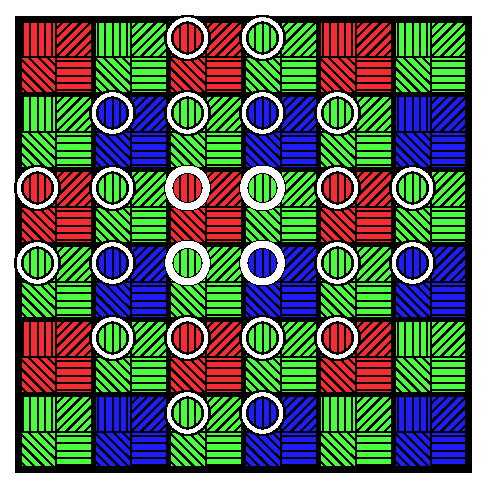
\includegraphics[width=.35\textwidth]{figures/polarized_image/normal_conv.pdf}
    \caption{Visualization of which pixels are used (white circle) to calculate the 6 YCbCr 4:2:0 values for the center \gls{cg} (thick white circle).}
    \label{fig:transformation}
\end{figure}